\documentclass[12pt,a4paper]{report}
\usepackage{szakd_report}

% SAJÁT
\parskip=12pt
\newcommand\tab[1][20pt]{\hspace*{#1}}
\usepackage{hyperref}
\usepackage{listings}
\lstset{
	basicstyle=\ttfamily\footnotesize,
	backgroundcolor=\color[rgb]{0.95,0.95,0.95},
	frame=single,
	tabsize=4,
	rulecolor=\color[rgb]{0.95,0.95,0.95},
	title=\lstname,
	escapeinside={\%*}{*)},
	breaklines=true,
	breakatwhitespace=true,
	framextopmargin=2pt,
	framexbottommargin=2pt,
	inputencoding=utf8,
	extendedchars=true,
	literate={á}{{\'a}}1 {é}{{\'e}}1 {í}{{{\'\i}}}1 {ó}{{\'o}}1 {ö}{{\"o}}1 {ő}{{\H o}}1 {ú}{{\'u}}1 {Ú}{{\'U}}1 {ü}{{\"u}}1 {ű}{{\H u}}1 {Ü}{{\"U}}1}
\graphicspath{{kepek/}}

\begin{document}
\pagestyle{empty} %a címlapon ne legyen semmi=empty, azaz nincs fejléc és lábléc

%A fõiskola logoja
{\large
\begin{center}
\vglue 1truecm
\textbf{\huge\textsc{Szakdolgozat}}\\
\vglue 1truecm

\epsfig{file=cimlap/ME_logo.eps, width=4.8truecm, height=4truecm}\\
\textbf{\textsc{Miskolci Egyetem}}
\end{center}}

\vglue 1.5truecm %függõleges helykihagyás

%A szakdolgozat címe, akár több sorban is
{\LARGE
\begin{center}
\textbf{CCRMS (Content \& Customer Relationship Management System), azaz online tartalom- és ügyfélkapcsolat-kezelő rendszer fejlesztése}
\end{center}}

\vspace*{2.5truecm}
%A hallgató neve, évfolyam, szak(ok), a konzulens(ek) neve
{\large
\begin{center}
\begin{tabular}{c}
\textbf{Készítette:}\\
Harkály Gergő\\
IV. évfolyam, Programtervező informatikus BSc.
\end{tabular}
\end{center}
\begin{center}
\begin{tabular}{c}
\textbf{Témavezetõ:}\\
Dr. Baksáné Dr. Varga Erika\\
Dr. Karácsony Zsolt
\end{tabular}
\end{center}}
\vfill
%Keltezés: Hely és év
{\large
\begin{center}
\textbf{\textsc{Miskolc, 2016. május 12.}}
\end{center}}

\newpage

\pagestyle{myheadings}
%Feladatkiiras
\begin{flushleft}
\textsc{\bfseries Miskolci Egyetem}\\
Gépészmérnöki és Informatikai Kar\\
Alkalmazott Matematikai Tanszék\hspace*{4cm}\hfil \textbf{Szám:}
\end{flushleft}
\vskip 0.5cm
\begin{center}
\large\textsc{\bfseries Szakdolgozat Feladat}
\end{center}
\vskip 0.5cm
Harkály Gergő (GOYLIZ) programtervező informatikus jelölt részére.\newline

\noindent\textbf{A szakdolgozat tárgyköre:} Web-alapú e-marketing eszköz fejlesztése\newline

\noindent\textbf{A szakdolgozat címe:} CCRMS (Content \& Customer Relationship Management System), azaz online tartalom- és ügyfélkapcsolat-kezelő rendszer fejlesztése\newline

\noindent\textbf{A feladat részletezése:}

\noindent Olyan komplex, web alapú megoldás létrehozása, mely egy áttekinthető és könnyen kezelhető felületen keresztül kiváltja a vállalkozások által értékesítésre és online marketingre jelenleg használt számos más programot. Az alkalmazás lehetőséget biztosít weboldal, esetleg webáruház létrehozására és tartalmi módosítására; hírlevelek írására és küldésére; látogatottsági, értékesítési és Google által biztosított statisztikák megtekintésére; rövidített linkek generálására; marketing-orientált megoldások alkalmazása (megosztó gombok, exit popup, RSS feed, regisztrációs űrlap, stb.) emellett a felhasználók vagy vásárlók adatainak nyilvántartására és a velük kapcsolatos interakciók követésére. A megoldás kidolgozása során az alábbi szempontokat szükséges figyelembe venni: keresőoptimalizálás, felhasználói élmény (UX), responsive design, moduláris felépítés, bővíthetőség, egyszerű fejlesztés, súgó.

\vfill

\noindent\textbf{Témavezető(k):} Dr. Baksáné dr. Varga Erika, adjunktus\newline

\noindent\textbf{Konzulens(ek):} Dr. Karácsony Zsolt\newline

\noindent\textbf{A feladat kiadásának ideje:} 2014. szeptember 30. \newline

%\noindent\textbf{A feladat beadásának határideje:}

\vskip 2cm

\hbox to \hsize{\hfil{\hbox to 6cm {\dotfill}\hbox to 1cm{}}}

\hbox to \hsize{\hfil\hbox to 3cm {szakfelelős}\hbox to 2cm{}}

\newpage

\vspace*{1cm}  
\begin{center}
\large\textsc{\bfseries Eredetiségi Nyilatkozat}
\end{center}
\vspace*{2cm}  

Alulírott Harkály Gergő; Neptun-kód: GOYLIZ a Miskolci Egyetem Gépészmérnöki és Informatikai Karának végzős Programtervező informatikus szakos hallgatója ezennel büntetőjogi és fegyelmi felelősségem tudatában nyilatkozom és aláírásommal igazolom, hogy CCRMS (Content \& Customer Relationship Management System), azaz online tartalom- és ügyfélkapcsolat-kezelő rendszer fejlesztése című szakdolgozatom/diplomatervem saját, önálló munkám; az abban hivatkozott szakirodalom felhasználása a forráskezelés szabályai szerint történt.

Tudomásul veszem, hogy szakdolgozat esetén plágiumnak számít:
\begin{itemize}
	\item szószerinti idézet közlése idézőjel és hivatkozás megjelölése nélkül;
	\item tartalmi idézet hivatkozás megjelölése nélkül;
	\item más publikált gondolatainak saját gondolatként való feltüntetése.
\end{itemize}

Alulírott kijelentem, hogy a plágium fogalmát megismertem, és tudomásul veszem, hogy plágium esetén szakdolgozatom visszautasításra kerül.

\vspace*{3cm}

\noindent Miskolc, 2016. év  05. hó 12. nap

\vspace*{3cm}

\hspace*{8cm}\begin{tabular}{c}
\hbox to 6cm{\dotfill}\\
Hallgató
\end{tabular}

\newpage

\noindent 1.

\begin{tabular}{cl}
&szükséges (módosítás külön lapon) \\
A szakdolgozat feladat módosítása& \\
& nem szükséges\\
&\\
\hbox to 4cm{\dotfill}&\multicolumn{1}{c}{\hbox to 5cm{\dotfill}}\\
dátum& \multicolumn{1}{c}{témavezető(k)}
\end{tabular}
\vskip1.5mm

\noindent 2. A feladat kidolgozását ellenőriztem:

\vskip1.5mm

\begin{tabular}{l@{\hspace*{4cm}}l}
témavezető (dátum, aláírás):& konzulens (dátum, aláírás):\\
\dotfill&\dotfill\\
\dotfill&\dotfill\\
\dotfill&\dotfill
\end{tabular}

\vskip1.5mm

\noindent 3. A szakdolgozat beadható:

\vskip1.5mm

\begin{tabular}{@{\hspace*{1.3cm}}c@{\hspace*{2.1cm}}c}
\hbox to 4cm{\dotfill}&\multicolumn{1}{c}{\hbox to 5cm{\dotfill}}\\
dátum& \multicolumn{1}{c}{témavezető(k)}
\end{tabular}

\vskip1.5mm

\noindent 4.
\begin{tabular}[t]{@{}l@{\hspace*{1mm}}l@{\hspace*{1mm}}l@{}}
A szakdolgozat& \hbox to 3.5cm{\dotfill} &szövegoldalt\\
              & \hbox to 3.5cm{\dotfill} &program protokollt (listát, felhasználói leírást)\\
              &\hbox to 3.5cm{\dotfill}   &elektronikus adathordozót (részletezve)\\
              &\hbox to 3.5cm{\dotfill} & \\
              &\hbox to 3.5cm{\dotfill} &egyéb mellékletet (részletezve)\\
              &\hbox to 3.5cm{\dotfill} &\\
\end{tabular}
\newline tartalmaz.

\vskip1.5mm

\begin{tabular}{@{\hspace*{1.3cm}}c@{\hspace*{2.1cm}}c}
\hbox to 4cm{\dotfill}&\multicolumn{1}{c}{\hbox to 5cm{\dotfill}}\\
dátum& \multicolumn{1}{c}{témavezető(k)}
\end{tabular}

\noindent 5.

\begin{tabular}{ll}
&bocsátható\\
A szakdolgozat bírálatra& \\
& nem bocsátható\\
\end{tabular}

\vskip1.5mm

\noindent A bíráló neve: \hbox to 8cm{\dotfill}

\vskip4mm

\begin{tabular}{@{\hspace*{1.3cm}}c@{\hspace*{2.1cm}}c}
\hbox to 4cm{\dotfill}&\multicolumn{1}{c}{\hbox to 5cm{\dotfill}}\\
dátum& \multicolumn{1}{c}{szakfelelős}
\end{tabular}

\noindent 6.
\begin{tabular}[t]{@{}l@{\hspace*{1mm}}l@{\hspace*{1mm}}l@{}}
A szakdolgozat osztályzata& &\\
&a témavezető javaslata:& \hbox to 3cm{\dotfill}\\
&a bíráló javaslata:& \hbox to 3cm{\dotfill}\\
&a szakdolgozat végleges eredménye:& \hbox to 3cm{\dotfill}
\end{tabular}

\vspace*{4mm}

\noindent Miskolc, \hbox to 4.5cm{\dotfill} \hspace*{2.5cm}
\begin{tabular}[t]{cc}
\hbox to 6cm{\dotfill}\\
a Záróvizsga Bizottság Elnöke
\end{tabular}
%feladat kiírás
\tableofcontents %automatikus tartalomjegyzék-változás esetén kétszer fordítani
\newpage
\pagestyle{fancy} %az oldal stílusa, ez adja az aláhúzott fejlecet
%Az elsõ fejezet
\Chapter{Bevezetés}
\label{Chap:bevezetes}

A napjainkban tapasztalható felgyorsult technikai fejlődés a webes környezetben is azonnali megoldásokat kívánt a programozóktól, részben ezért is született már számos fejlesztőkörnyezet. Az internetnek köszönhetően pedig több, egymástól távol élő szoftverfejlesztő tud együtt dolgozni, valamint az ő munkájukat önkéntes, a programozás iránt érdeklődő személy segíteni, észrevételeikkel, visszajelzéseikkel támogatni. Így születhetett meg számos ingyenes, nagy tudással bíró, interneten keresztül letölthető tartalomkezelő rendszer is, ismertebb nevén CMS, mely az angol Content Management System szavakból álló mozaikszóról kapta a nevét.

Ezek közül a legismertebbek betűsorrendben: Drupal, ExpressionEngine, Joomla, Magento, OpenCart, PrestaShop, WordPress. Emellett természetesen az informatikai vállalkozások többsége is kifejlesztett már saját tartalomkezelő rendszert, melyek kereskedelmi forgalomban nem elérhetőek.

A CMS-ek segítségével akár egy néhány perces, szinte automatikus telepítést követően már kész adminisztrációs felületet, webes szolgáltatásokat, sablonokat és kiegészítőket kap a szoftver használója. Többségük a tartalom felvitelén és módosításán túl olyan további funkciókat is biztosít, mint hozzászólási lehetőség az egyes bejegyzésekhez, médiatár, hírlevélküldés vagy akár kész webáruház kialakítása kosárral és fizetési modulok integrálásával.

A kommunikációs csatornák (telefonhívás, sms, e-mail, honlap, stb.) kiszélesedésével és a webáruházak létrehozásának leegyszerűsödésével lényegében kinyílt a világ a vállalkozások előtt. A széles spektrumú értékesítési csatornák természetesen az ügyfélkör növekedését is magukkal vonták, ezért a korábban működőképes, kizárólag ismeretségi vagy helybeli közelségre alapuló értékesítési megoldások mára kevésbé alkalmazhatóak. A felhasználók, vásárlók naponta rengeteg ingert kapnak, emellett végzettségük, fizikai távolságuk és egyéb jellemzőik alapján teljesen eltérően kezelendőek. Így új megoldások születtek a felhasználók adatainak nyilvántartására és a vállalkozást is támogatni képes kezelésére, melyek napjainkban még kevésbé terjedtek el. Ezeket az eszközöket nevezi a szakma CRM rendszereknek, mely az angol Customer Relationship Management, azaz ügyfélkapcsolat-kezelőre utal. Az egyik leghíresebb magyar megoldás a miniCRM, míg az Oracle hasonló webes megoldása - mely inkább nagyvállalatok körében elterjedt - a Siebel, számos nemzetközi vállalkozás pedig a Salesforce rendszerét használja.

A CRM lényege, hogy a felhasználókról, vásárlókról, illetve a velük történő interakciókról szinte minden adatot és iratot nyilván lehet tartani, azokból statisztikákat készíteni, a statisztikákból pedig célirányosabb marketinget végezni. A személyes adatok mellett akár a szerződések és egyéb dokumentumok feltöltésére, visszakeresésére is alkalmas, továbbá rögzíthetőek a kapcsolatfelvétel időpontjai és eseményei, függetlenül attól, hogy az adott interakciót melyik fél kezdeményezte. Ennek köszönhetően teljes körű ügyféltörténet bontakozik ki a CRM használója előtt, hisz akár pontosan látja például, hogy az adott vevő mikor látogatott el utoljára az üzletbe, ott mi után érdeklődött, milyen kérdései voltak, kötött-e szerződést, ha igen, azon mi szerepel, hívta-e azóta az ügyfélszolgálatot, és még sorolhatnánk.

\Section{Motiváció}

%A meglévő tartalomkezelő rendszerek - bár rendkívül sok opciót foglalnak magukban, mégis - a hosszú távú működésben gondolkodó informatikai vállalkozásoknak nem biztosítanak megfelelő hátteret. Nem véletlen, hogy a vállalatok többsége vagy egyszerre vesz igénybe több apró szolgáltatást, s biztosítja így a működéshez szükséges minden funkciót, vagy saját fejlesztésű megoldásokkal dolgozik, ugyanis a külső, más fejlesztői csoportoktól való függőség számos problémát felvet. Ahhoz, hogy a jelenleg is elérhető CMS-ekkel az ügyfelek igényeit széles körben ki lehessen szolgálni, több kiegészítőt, úgynevezett plugint szükséges telepíteni, vagy saját magunknak fejleszteni. A mások által készített és általunk telepített eszközök azonban nem mindig megfelelően integrálódnak az egyéni érdekek alapján módosított alapverziókhoz.

%Emellett mind a CMS, mind a CRM önmagában olyan bonyolult struktúrájú, hogy alapvetően ezeket külön fejlesztések és szoftverek formájában szokás használni. Bár össze lehet őket kapcsolni, esetleg bővítményként telepíteni egyiket a másikba, azonban nem elterjedt olyan megoldás, ahol a szoftver alapvetően úgy épülne fel, hogy mindkét opciót alapértelmezetten tartalmazza.

%Ezért döntöttem amellett, hogy marketingorientált megközelítést alkalmazva, a meglévő tapasztalatokra alapozva olyan tartalomkezelő rendszert hozok létre, mely egy weboldal és/vagy webáruház tartalmi kiszolgálása mellett képes ellátni az ügyféladatbázis nyilvántartását és kezelését is.

A feladat egy Európai Uniós projekt keretében valósulhatott meg, mely során a "Közép-dunántúli kerékpáros turisztikai hálózat" című pályázatban foglaltaknak megfelelően kellett kialakítani mind a megjelenést, mind a működést. Az elkészült website a \url{http://www.katt.sport.hu} domain név alatt tekinthető meg, mivel a Tatabányai Alpin Sportklub, mint pályázó vezetése a jelenleginél is nagyobb víziókban gondolkodva a Közép-dunántúli Aktív Turisztikai Térség szavakból képzett KATT mozaikszóval illette a projektet.

Az ajánlatkérésben foglalt elvárások meghatározó módon befolyásolták, korlátozták a felhasználható alternatívákat:
\begin{itemize}
	\item A későbbiek folyamán lehessen könnyen továbbfejleszteni az oldalrendszert.
	\item Az oldalrendszer képes legyen kezelni legalább 120.000 karakter szöveget és 2000 db digitális fotót.
	\item A fenntartási időszak végéig vállaljanak garanciát az oldal programozására.
	\item Tudjunk eseményeket megjeleníteni is, és ezeket mi tudjuk frissíteni.
	\item Több admin személyt is kinevezhessünk, és megfelelő jogosultság birtokában frissíthessék az oldal tartalmát.
\end{itemize}

A továbbiakban bemutatandó tartalomkezelők közül a WordPress bizonyult a leginkább megfelelőnek, hiszen már az alaprendszer is képes számos igényt kielégíteni, így például a meglévő tartalmak egyszerű, grafikus felületen keresztüli módosítási lehetőségét, képek feltöltését, módosítását (Médiatár). Mivel a WP a legelterjedtebb nyílt forráskódú CMS, így a későbbi továbbfejlesztés sem jelent majd akadályt, valamint a hosszú távú biztonságos és korszerű fenntartása is biztosított a közösségnek hála. Felhasználói jogosultsági szintekből pedig öt beépítetttel is rendelkezik: feliratkozó (subscriber), közreműködő (contributor), szerző (author), szerkesztő (editor) és adminisztrátor (administrator), szükség esetén azonban további szintek is deklarálhatóak.
\Chapter{Létező rendszerek főbb ismérvei}
\label{Chap:tema}

A jelenleg interneten elérhető tartalomkezelő rendszereknek épp úgy megvannak a hátrányai is, mint amennyire előnyösek. Többségük ingyenesen elérhető, valamint nyílt forráskódúak, s bár ez mindenképpen pozitív a webfejlesztők számára, épp annyi bosszúságot is okoz. A nyitottságnak köszönhetően a hackerek is részletesen megismerhetik e programkódokat, a hibáikat, így nem ritka a kizárólag egy-egy CMS ellen irányuló támadás. Évről-évre előfordul, hogy számos olyan weboldal esik úgynevezett brute force-támadás áldozatául, melyeket az ismertebb rendszerek (például Joomla vagy WordPress) szolgálnak ki.

Emellett amennyiben az adott weboldal tartalmaihoz a látogatók számára hozzászólási lehetőség is biztosított, az űrlapon gyakran tesznek közzé spamet, hirdetést az erre kifejlesztett robotok (úgynevezett "spambot"-ok). Természetesen captcha segítségével van mód a védekezésre, ám az korántsem tökéletes.

Ezen rendszerek további hátránya, hogy a megfelelő beállításhoz és használathoz a fejlesztőnek, az üzemeltetőnek és végfelhasználónak is el kell sajátítania, meg kell ismernie azt. Könnyen belátható, hogy az egyedi igények alapján fejlesztett saját rendszer módosítása és beállítása jóval egyszerűbb, mint egy általános célú, mások által létrehozotté.

Fontos kihangsúlyozni azonban, hogy a fenti hátrányok ellenére az informatikai szakemberek is elismerik ezeket az eszközöket, ezért is oly gyakori a használatuk, például a Facebook Newsroom és a Google Ventures WordPress, a ShopRenter.hu, mint magyarországi, webáruház bérlésre szakosodott vállalkozás rendszere OpenCart alapokon nyugszik. Emellett számos, az ismertebb tartalomkezelőkkel dolgozó vállalkozás jelent meg az elmúlt években, lényegében már néhány ezer forintért vásárolhatunk kész fordításokat, kiegészítőket és sablonokat.

\newpage

\Section{Drupal}

\begin{figure}
	
\includegraphics[width=1\textwidth]{cms-drupal-org.png}
	\caption{A drupal.org főoldala}
\end{figure}

A (\href{https://www.drupal.org/}{Drupal}) leginkább a nagyvállalatok vagy intézmények körében elterjedt. Rendkívül sokoldalú, ám hatalmas tárigénnyel rendelkezik. Tekintettel arra, hogy a telepítést követően az alap adatbázis is már önmagában több megányi adatot tartalmaz, a rendszer első használat előtti teljes körű megismerése sok időbe és energiába telik. Leginkább állami, önkormányzati vagy iskolai weboldalak kiszolgálására használják.

A \href{https://www.drupal.hu/kezikonyv/tkr}{Drupal.hu leírása}:

\begin{quote}
"A Drupal 2001. január tizenötödikén kezdte meg nyílt működését, amikor Dries Buytaert publikálta első verzióját az interneten. A rendszer azóta nagyon sokat fejlődött, és széles körben használt tartalomkezelővé vált.

\dots

A Drupal egy eléggé vékony réteget biztosít a PHP nyelvi elemei felett, mely jelentősen meg tudja könnyíteni általánosabb igényű web alkalmazások fejlesztését. Ilyen funkciók az általános űrlapkezelő rendszer, a vékony adatbázis kezelő réteg, a felhasználókezelő alrendszer."
\end{quote}

\newpage

\Section{Joomla}

\begin{figure}
	
\includegraphics[width=1\textwidth]{cms-joomla-org.png}
	\caption{A joomla.org főoldala}
\end{figure}

A több, mint 50 millió letöltéssel rendelkező \href{https://www.joomla.org/}{Joomla} talán a második leginkább keresett honlapmotor. A szoftver filozófiája az, hogy az adminisztrációs felületen keresztül, külön programozás nélkül is számos feladatot el lehessen végezni. Nem véletlen tehát, hogy a webfejlesztéshez kevésbé értő személyek örömmel használják e CMS-t. Ám a sokszínű megoldás alapértelmezett mivoltának van hátránya is: programozói oldalról egy-egy fejlesztés komoly szaktudást igényel. Erősen alapszik az XML-re és a névterekre, az adminisztrációs felület biztonságára pedig különösen nagy hangsúlyt fektet.

A \href{http://joomlacms.hu/joomla/mi-a-joomla}{joomlacms.hu} leírása:

\begin{quote}
"A Joomla egy ingyenes és nyílt forráskódú tartalomkezelő rendszer (Content Management System), ami saját modell-nézet-vezérlőből (MNV) és különböző népszerű webes keretrendszerek alkalmazásából áll.

Ezeknek a technológiáknak a segítségével könnyedén oszthatunk meg különböző típusú tartalmakat a világhálón és a helyi intraneten egyaránt. Maga a Joomla! objektum-orientált programozási (OOP) szemléletet követ a fejlesztők által bevezetett szoftvertervezési minta alapján, mind ezt PHP nyelven. Az adatok tárolása MySQL-ben vagy egyéb támogatott adatbázisban történik.

Maga a rendszer egy nagy közösség által fejlesztett moduláris termék, melynek a komponenseit úgy állították össze, hogy a legszélesebb körök igényeit is kielégítse, továbbá lerövidítse az üzembe helyezést, valamint a tartalom felvitelének idejét. \dots A Joomla bővítményletöltő weboldalán több ezer bővítmény várja a felhasználókat."
\end{quote}

\newpage

\Section{Magento}

\begin{figure}
	
\includegraphics[width=1\textwidth]{cms-magento-com.png}
	\caption{A magento.com főoldala}
\end{figure}

A \href{http://magento.com/}{Magento} egy eBay Inc. fejlesztésű webáruházmotor. Bár a korábbi verziókhoz készült magyar nyelvű fordítás, azok az új kiadásokkal nem, vagy nem teljesen kompatibilisek. Alapvetően két különálló fejlesztés érhető el: egy ingyenes, kevesebb szolgáltatást tartalmazó (Community Edition), és egy díjköteles verzió (Enterprise Edition). Aki komolyabb webáruházban gondolkodik, mindenképpen célszerű kipróbálnia ezt a rendszert is, hiszen rendkívül sok funkcióval bír, és nagyszerű megoldásokat alkalmaz az adminisztráció ellátásához, valamint a megfelelő üzemeltetéshez.

A \href{http://magentoshop.hu/a-magento-keretrendszerrol/}{magentoshop.hu} leírása:

\begin{quote}
"A Magento egy nyílt-forráskódú e-commerce fejlesztési keretrendszer, amelyet jelenleg több ezer fejlesztő használ és gondoz világszerte.

\dots

A Magento egy olyan portálmotor, amely kifejezetten webáruház-funkcio- nalitás magas szintű kiszolgálására készült. Egy olyan rendkívül fejlett e-kereskedelemi keretrendszer, amely ingyenesen hozzáférhető, és amelyre\\ frontend felületet fejlesztve egy rendkívül funkciógazdag webáruházat készíthetünk.

A Magento a világ egyik vezető webáruház-motorja. Több tízezer nagy terhelhetőségű, komplex webshopot szolgál ki a világ minden táján és folyamatosan fejlődik."
\end{quote}

\newpage

\Section{OpenCart}

\begin{figure}
	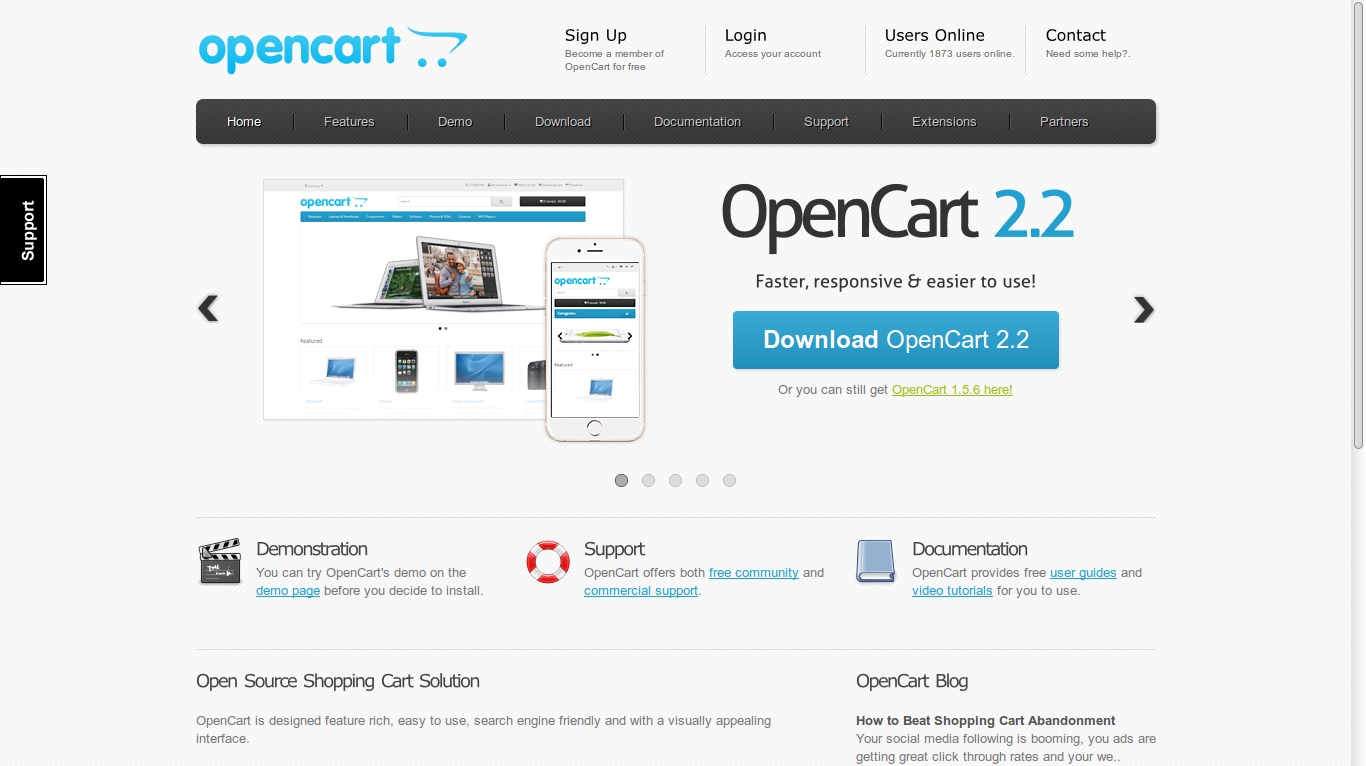
\includegraphics[width=1\textwidth]{cms-opencart-com.png}
	\caption{A opencart.com főoldala}
\end{figure}

Az \href{http://www.opencart.com/}{OpenCart} az ingyenesen elérhető webáruházmotorok közül talán a leginkább ismert és ezért leginkább használt. Bár évek óta jelen van a piacon, a második (OpenCart 2.0), már responsive verziója mégiscsak 2014. év végén jelent meg. A magyar nyelvű változat más CMS-ekkel ellentétben (Joomla, WordPress) még kevésbé kidolgozott. A szoftver talán legnagyobb hátránya, hogy tökéletesen csak webshop létrehozására alkalmas, s bár telepíthetőek különböző kiegészítők a nagyobb spektrumú használathoz, azok csak minimális szolgáltatást biztosítanak. Így például az OpenCart alapú webáruházhoz megfelelő minőségű és szolgáltatású Blog vagy Hírek aloldalt szinte lehetetlen létrehozni.

Az \href{http://www.opencart-hungary.hu/}{open-cart-hungary.hu} leírása:

\begin{quote}
"Az OpenCart egy funkciógazdag, könnyen kezelhető, keresőbarát és egy tetszetős admin felülettel ellátott webáruház rendszer.

\begin{itemize}
	\item korlátlan kategória, termékszám és gyártó kezelés
	\item többféle valuta használható
	\item többnyelvű kezelőfelület
	\item véleményezhető termékek és termék értékelő
	\item sablonokkal átváltoztatható arculat
	\item több mint 20 fizetési modul
	\item több mint 8 szállítási modul
	\item magyar nyelvű kiegészítők és modulok"
\end{itemize}
\end{quote}

\newpage

\Section{PrestaShop}

\begin{figure}
	
\includegraphics[width=1\textwidth]{cms-prestashop-com.png}
	\caption{A prestashop.com főoldala}
\end{figure}

A \href{http://www.prestashop.com/}{PrestaShop} webáruházmotor fejlesztését Franciaországban kezdték el, majd számos országból csatlakoztak a kezdeményezéshez, így hozva létre több nyelven is a rendszert. Egy webshop funkcióit maximálisan képes ellátni.

A \href{https://hu.wikipedia.org/wiki/PrestaShop}{Wikipédia szócikke} alapján:

\begin{quote}
	"A PrestaShop az Open Software License 3.0-s verziója alapján kiadott nyílt forráskódú e-kereskedelmi webes alkalmazás. Alapítói Igor Schlumberger és Bruno Léveque. Rugalmas és moduláris architektúrájának köszönhetően egyre nagyobb népszerűségre tesz szert. Egyszerűbb, de ugyanakkor gyorsabb, mint a Magento.

	A PrestaShop alapítása 2005-re nyúlik vissza. Öt ifjú egyetemi hallgató fogott össze az Epitech informatikai iskolában. A két nyelven (francia és angol) kiadott eredeti projektnek a phpOpenStore (POS) nevet adták. Alapítói úgy döntöttek, hogy szabad szoftverként teszik hozzáférhetővé. Számos kiskereskedő vett részt a tesztelésben és a rendszerkövetelmények meghatározásában.

	A PrestaShop felhasználói az alapkonfiguráció paraméterein kívül több szinten testre szabhatják a rendszert:
	\begin{itemize}
		\item a PHP-ismeretekkel rendelkező felhasználók az igényeiknek megfelelően tudják módosítani a programkódot;
		\item a PrestaShop felhasználói saját grafikai arculatot tervezhetnek;
		\item szolgáltatások bővítése: telepíthető, konfigurálható és szükség esetén letiltható modulok formájában lehetséges;"
	\end{itemize}
\end{quote}

\newpage

\begin{figure}
	
\includegraphics[width=1\textwidth]{crm-minicrm-hu.png}
	\caption{A minicrm.hu főoldala}
\end{figure}

\Section{MiniCRM}

A \href{http://www.minicrm.hu/}{MiniCRM} egy ügyfélkezelési rendszer sikeres kisvállalatoknak. Segít hatékonyan feldolgozni az érdeklődéseket, optimalizálni az értékesítési folyamatot, még több sikeres értékesítést lezárni.

Az alapítók (köztük leginkább Leskó Norbert) fejében 2006-ban fogalmazódott meg a CRM rendszer gondolata, mikor saját cégük ügyfélkapcsolatait igyekeztek a lehető leghatékonyabban kezelni. 2009 óta kizárólag a MiniCRM fejlesztésével és üzemeltetésével foglalkoznak, ami 2010-ben önálló termékként került a piacra.

A cég 2012 óta folyamatosan bővül. A munkaterületeket minden eddiginél részletesebben osztották fel, így specializálódott munkatársaik még hatékonyabban tudják segíteni ügyfeleik munkáját. A MiniCRM-et is folyamatosan fejlesztik, hogy átfogóan kielégítse a kis- és középvállalkozások igényeit.

A kitartásnak meglett az eredménye: a MiniCRM 2014-ben elnyerte a Deutsche Telekom "Legjobb üzleti app" díját, melynek köszönhetően 2015. márciustól megkezdhették terjeszkedésüket a régióban, a tervek között Horvátország, Szlovákia, Románia és Lengyelország szerepel. Ennek hála a jelenleg kizárólag magyarokból álló csapat más nemzetiségű munkatársak felvételét is tervezi.

\begin{quote}
"A CRM több, mint egy szoftver. Olyan szemléletmód, amely a vállalat legfontosabb tőkéjét állítja középpontba: az ügyfeleket. Használatával lépésről lépésre lehet a hírlevél feliratkozóból komoly érdeklődőt generálni, a komoly érdeklődőt hatékonyan lezárni, valamint a korábbi vevőknek újra eladni, egyszóval: cégértéket építeni az ügyfelekből." (forrás: \href{http://www.minicrm.hu/tour/crm/}{minicrm.hu})
\end{quote}

\newpage

\Section{Siebel}

\begin{figure}
	
\includegraphics[width=1\textwidth]{crm-oracle-com-siebel.png}
	\caption{Az oracle.com Siebel aloldala}
\end{figure}

A \href{http://www.oracle.com/siebel}{Siebel CRM} nevét az 1993-ban alapított Siebel CRM Systems Inc. fejlesztőjéről, Thomas Siebel-ről kapta. A vállalkozást 2005-ben felvásárolta az Oracle.

A Siebel egy web-alapú megoldás az ügyféladatok nyilvántartására és kezelésére. Használata leginkább a nemzetközi nagyvállalatok körében elterjedt, mivel az alapprogram egyedi igényeknek megfelelő átalakítása jelentős költséget von maga után.

Magyarországon a Magyar Telekom Nyrt. használta hosszabb ideig, a Vodafone Magyarország Zrt. pedig évekkel ezelőtt elindította az áttérést e rendszerre.

A \href{http://www.trilobita.hu/termekek/viszonteladott-termekek/oracle-alkalmazasok/oracle-siebel-crm}{trilobita.hu} bemutatkozó leírása:

\begin{quote}
"Az Oracle Siebel CRM területen a világ egyik legátfogóbb megoldását nyújtja elsősorban olyan nagy méretű vállalatok számára, ahol a kereskedelmi és/vagy marketing tevékenység az üzleti működés szempontjából meghatározó szereppel bír.

\dots

Legfőbb referenciánk ezen a területen a Credigen Bank Zrt.-nél 2009-ben történt Siebel bevezetés, ahol a fő hangsúly a marketing kampányok teljeskörű támogatásán és az elemző funkciókon volt. A rendszert továbbá integráltuk a bank Call Center megoldásávál, ezáltal  a marketing kampányok végrehajtását is megtámogatva."
\end{quote}

\newpage

\Section{WordPress}

\begin{figure}
	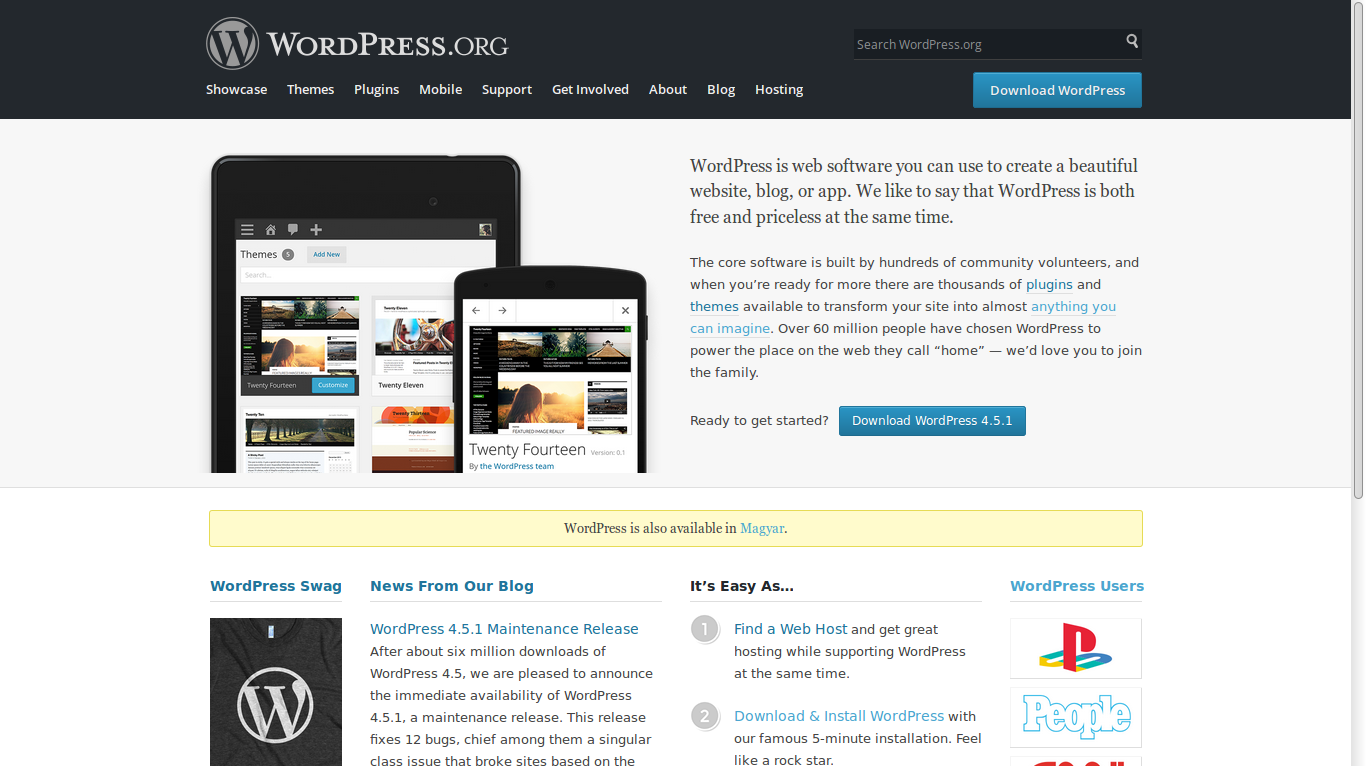
\includegraphics[width=1\textwidth]{cms-wordpress-org.png}
	\caption{A wordpress.org főoldala}
\end{figure}

A \href{https://wordpress.org/}{WordPress} napjaink egyik legelterjettebb tartalomkezelő rendszere, több tízmillió aktív weboldalt szolgál ki. Az egyedileg telepíthető eszköz a \href{https://wordpress.org/}{wordpress.org} oldalról tölthető le, míg a \href{https://wordpress.com/}{wordpress.com} honlapon egy regisztrációt követően azonnal, díjmentesen használatba is vehetjük a CMS szolgáltatásait, blogot vezethetünk, honlapot üzemeltethetünk.

A fordítások szinte minden nyelven elérhetőek, továbbá számos bővítmény (plugin) és sablon (theme/template) érhető el ingyenesen, valamint fizetős verzióban is.

A WordPress-t Matt Mullenweg (\href{http://ma.tt/}{ma.tt}), a houstoni egyetem első éves hallgatója kezdte el kifejleszteni 19 éves korában. Rendszeresen blogolt a b2/cafelog (\href{http://cafelog.com/}{cafelog.com}) alapú honlapján, ám ahogy növekedett a weboldal látogatóinak száma, egyre inkább szükségét érezte egy megbízhatóbb rendszer megalkotásának. 2003-ban létrehozta a WordPress (röviden: WP) első verzióját, mely mára a világ vezető blogmotorjává vált, 2012. márciusában 72.4 millió WP-alapú oldal létezett.

A \href{https://hu.wordpress.org/}{hu.wordpress.org} leírása:

\begin{quote}
"A WordPress egy modern publikációs platform, amely az esztétikát, a webes szabványokat, és a használhatóságot tartja szem előtt. A WordPress egyszerre ingyenes és szabadon felhasználható.

Egyszerűbben, a WordPress arra való, hogy publikálj, és nem arra, hogy harcolj vele."
\end{quote}

\newpage

\Chapter{Problémák elméleti megközelítése}
\label{Chap:problemak}

A feladat elvégzése során, mint ahogy az a projekteknél megszokott, számos kérdés vetődött fel, melyekre megoldást kellett találni. Egy-egy kérdéses elemre nyilvánvalóan több válasz is adható, így igyekeztem megtalálni a legmegfelelőbbet mind közül.

\Section{Használandó technológiák}

Első és legnagyobb kérdés a használandó technológiák kiválasztása. Döntésemnél figyelembe vettem azt, hogy manapság melyik rendszer mennyire elterjedt, emiatt hosszú távon is piacképes, valamint azt, hogy mennyire dokumentáltak, így könnyen találni már meglévő megoldásokat, valamint kiindulási pontot a hibaelhárítások során (debug). Emellett nem kerülhettem el azt a tényt sem, hogy a mobilos (ide értve a tabletet is) internethasználat rohamos léptekben terjed, ezért mind az adminisztrációs felület, mind a design tekintetében erre szinte kötelező jelleggel fel kell készülni.

\SubSection{Tartalomkezelő rendszer kiválasztása}

A WordPress egy kész tartalomkezelő rendszer, melyet - mint ahogy azt a bevezetőben bemutattam - a világ számos pontján, szinte a gazdaság bármely területén tevékenykedő vállalkozás használ jelenleg is, hiszen több tízmillió weboldal jött létre segítségével.

Ennek köszönhetően mind a felhasználói, mind a fejlesztői dokumentáció rendkívül részletes, mely nagyban megkönnyíti a projekt kivitelezését, valamint a későbbi módosítási kérések gyors és hatékony lekezelését.

A WordPress adatbázisának, valamint az adminisztrációs felületének felépítése - összehasonlítva más ingyenesen elérhető alternatívákkal, melyeket szintúgy taglaltam e dolgozat elején - bizonyult a legcélravezetőbbnek. Míg a webáruházra szolgáló rendszerek (így például Magento) a termékadatok tárolására a jelenlegi igényeknél bőven túlmutató, rendkívül összetett struktúrát valósítanak meg, addig a WordPress + WooCommerce kombináció alig néhány táblával bővíti ki a MySQL adatbázist.

\begin{figure}[H]
	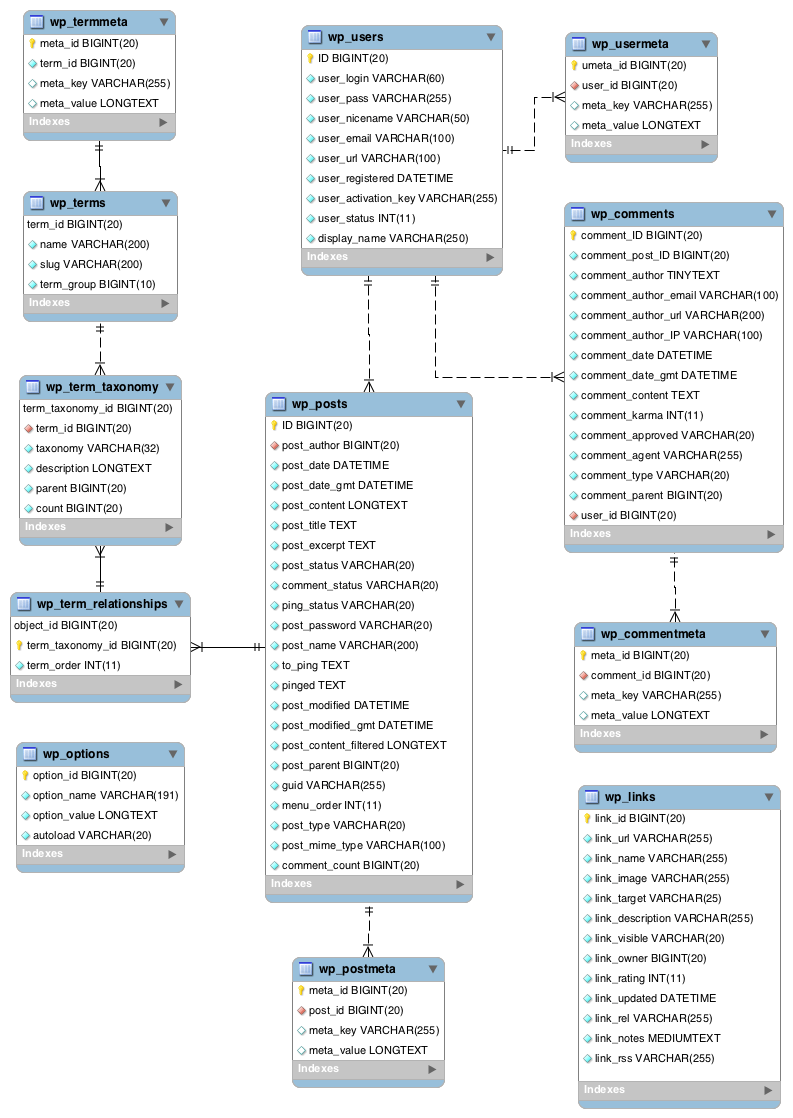
\includegraphics[width=1\textwidth]{wordpress-ER-diagram.png}
	\caption{A WordPress 4.4.2 ER diagramja (forrás: https://codex.wordpress.org/Database\_Description)}
\end{figure}

\Section{Egyedi adatstruktúra szervezése}

A tárolandó, illetve használandó adatok esetében is vetődtek fel kérdések, így például a névnapi köszöntő megtervezésekor is. Egyrészt szerettem volna automatikus üzeneteket küldeni, tehát az év minden napjához el kellett tárolnom a hivatalos magyarországi névnapokat, ahol több is van egy nap, ott természetesen mindegyiket. Ekkor keresésnél a dátum jelentené az indexet. Emellett szerettem volna könnyíteni a felhasználók dolgát is azzal, hogy a keresztnév megadásakor automatikusan felajánlom az adott névhez társítható dátumokat (hiszen egy-egy névből nemcsak egy, hanem több névnap is lehet egy éven). Ebben az esetben a keresések során az index már maga a név lenne, s nem a dátum. Ez ellentmondáshoz vezetett.

Megoldási alternatíva több is adódott előttem. Egyrészt a switch-case szerkezet, másrészt a tömbök, harmadrészt az adatbázis. Figyelembe véve azt, hogy önmagában a magyar keresztnevekből több, mint 4000 van, a switch-case szerkezetet elvetettem, mert ebben az esetben már lassú lett volna a keresés, hisz ott az értékek nincsenek indexelve, a program egyszerű összehasonlítást végez. Azt is mérlegeltem, hogy nem olyan adatokról van szó, melyeket védeni kellene, ezért az adatbázisban történő tárolása értelmetlennek és feleslegesen biztonságosnak tűnt. Ezért a tömb mellett döntöttem, hiszen bár a PHP nyelvben nincs úgynevezett HashMap, mint más fejlett programozási nyelvekben (például Java), a tömb megvalósítása lényegében megfelel annak.

\SubSection{PHP tömb, mint hasítótáblás leképezés}

A \href{http://php.net/manual/en/language.types.array.php}{php.net} hivatalos magyarázata a tömbről:

\begin{quote}
"An array in PHP is actually an ordered map. A map is a type that associates values to keys. This type is optimized for several different uses; it can be treated as an array, list (vector), hash table (an implementation of a map), dictionary, collection, stack, queue, and probably more. As array values can be other arrays, trees and multidimensional arrays are also possible."
\end{quote}

Mindez szabad fordításomban:

\textit{A PHP tömb valójában egy hasítótáblás leképezés (HashMap), mely egy olyan adattípus, ami kulcsokhoz rendel értékeket. Ez a megoldás számos különböző felhasználásnak megfelel, hiszen kezelhető tömbként, listaként (vektor), hasítótáblaként (a leképezés egy megvalósítási formája), halmazként, sorként, és még sorolhatnánk. Mint ahogy a tömbök állhatnak további tömbökből, ugyanúgy lehetséges a fa adatszerkezet és a többdimenziós tömb is.}

\newpage

Példa PHP tömbre:
\begin{lstlisting}
<?php
$tomb = array(
	"kulcs1" => "ertek1",
	"kulcs2" => "ertek2",
);
// PHP 5.4 felett
$tomb = [
	"kulcs1" => "ertek1",
	"kulcs2" => "ertek2",
];
\end{lstlisting}

\Section{Layout tervezés}

A weboldalt, webalkalmazást jó esetben nem magának készítteti a megrendelő, hanem a vásárlóinak, ügyfeleinek, ám a saját céljai elérése érdekében. Ezt a két érdekkört kellett a design megtervezése során figyelembe vennem, tehát olyan megjelenést kialakítani, ami mind a látogatóknak, mind az üzleti tevékenységnek megfelel.

Mivel a weboldalak jelentős részén a menüpontok egy felső vízszintes sávban helyezkednek el, így azzal a feltételezéssel éltem, hogy a felhasználók többsége is - márcsak megszokásból is - itt fogja keresni, ennek megfelelően ott helyeztem el.

\begin{figure}[H]
	
\includegraphics[width=1\textwidth]{katt-sport-hu-fooldal.jpg}
	\caption{A katt.sport.hu tervezett főoldalának felső része}
\end{figure}

\newpage

Egy honlapot véleményem szerint két fő okból keresnek fel: további információ szerzése az adott vállalkozásról, annak tevékenységéről, termékeiről (esetleg azok igénylése, megvásárlása), másrészt a kapcsolati adatok (telefonszám, e-mail cím, telephely) és nyitvatartási rend miatt. Tekintettel a mobiltelefonos böngészés terjedésére az elérhetőségek a lap legtetején kerültek megjelenítésre, így kisebb kijelzőn ezek az adatok jelennek meg azonnal a felhasználóknak.
\Chapter{Fejlesztői dokumentáció}
\label{Chap:dokumen}

\Section{WordPress, mint a rendszer alapja}

A feladatot WordPress tartalomkezelő rendszer, illetve a most már szintúgy \href{https://automattic.com/}{Automattic} tulajdonában lévő \href{https://wordpress.org/plugins/woocommerce/}{WooCommerce} webáruház bővítmény segítségével valósítottam meg. Ezekre alapozva építettem meg egy kívánt és szükséges funkciókat tartalmazó plugint, valamint a weboldal megjelenését szolgáló sablont.

A  \href{https://wordpress.org/download/}{WordPress angol nyelvű alapcsomagjában} található Akismet és Hello Dolly kiegészítőket, valamint a Twenty Fourteen, Fifteen és Sixteen sablonokat (melyek egyébként a kiadás évét jelölik: 2014, 2015, 2016) eltávolítottam, a \href{https://hu.wordpress.org/}{magyar telepítőcsomagból} pedig áthelyeztem a nyelvi fájlokat tartalmazó \verb|/wp-content/languages| mappát a szükségtelen plugin és sablon nyelvi fájlok nélkül.

Ezt követően a \texttt{/wp-content/themes} mappában létrehoztam a saját fejlesztésű sablon mappáját \texttt{CCRMS-theme} néven, a \texttt{/wp-content/plugins} mappában pedig a \texttt{CCRMS-plugin} nevű mappát a tervezett bővítményhez.

Bővítmény esetében elegendő egy \verb|index.php| fájl egy minimális fejléccel és máris egy használható, bekapcsolható plugin lesz belőle, míg a sablon esetében az \verb|index.php| fájl mellett egy \verb|style.css| fájlra is szükség van, melynek fejlece szintúgy kötött.

A bővítmény fejlece (index.php):
\begin{lstlisting}
<?php
/*
Plugin Name: CCRMS Plugin
Plugin URI: http://users.iit.uni-miskolc.hu/~harkaly
Description: Content & Customer Relationship Management System plugin
Version: 2016.05.01.
Author: Harkály Gergő GOYLIZ
Author URI: http://users.iit.uni-miskolc.hu/~harkaly
Text Domain: ccrmsplugin
*/
\end{lstlisting}

A sablon stíluslapjának fejlece (style.css):

\begin{lstlisting}
/*
Theme Name: CCRMS Theme
Theme URI: http://users.iit.uni-miskolc.hu/~harkaly
Version: 2016.05.01.
Author: Harkály Gergő GOYLIZ
Author URI: http://users.iit.uni-miskolc.hu/~harkaly
Description: Content & Customer Relationship Management System WordPress Template
License: All rights reserved!
License URI: http://users.iit.uni-miskolc.hu/~harkaly
Tags: responsive
Text Domain: ccrmstemplate
*/
\end{lstlisting}

A \texttt{textdomain}-ről még a későbbiekben szó lesz, előljáróban annyit, hogy ez járul hozzá a sablon, illetve az egész honlap egyszerű többnyelvűsítéséhez.

\newpage

\Section{Biztonság}

A weboldal, illetve a rendszer biztonságosságát kritikus pontnak tekintettem, ennek érdekében igyekeztem mindent meg is tenni.

A WordPress adminisztrációs felülete a \texttt{/wp-login.php} vagy \texttt{/wp-admin} URL-eken érhető el, bár mindkét esetben valójában a \texttt{/wp-admin} mappa tartalma biztosítja a kezelőfelületet. Éppen ezért a \texttt{/wp-admin} mappát, így a belépési lehetőséget is egy \texttt{.htaccess}, \texttt{.htpasswd} párosítással korlátoztam le. Tehát a \texttt{wp-admin} mappában elhelyeztem egy \texttt{.htaccess} fájlt az alábbi kóddal:

\begin{lstlisting}
<Files admin-ajax.php>
	Order allow,deny
	Allow from all
	Satisfy any
</Files>

AuthName "admin + 1234"
AuthType Basic
AuthUserFile /path/to/.htpasswd
Require valid-user
\end{lstlisting}

A \texttt{wp-admin} mappában található \verb|admin-ajax.php| fájlra szüksége van több WordPress funkciónak is, ezért arról le kell venni a korlátozást, ezt  a kód első része biztosítja. Az \texttt{AuthName} által egyes böngészőkben meg is jelenik, hogy pontosan mit kell a felhasználónak beírni a felugró ablakba (admin, 1234), azonban ez kellő biztosítéknak bizonyult ahhoz, hogy megállítsa a robotokat, illetve az illetéktelen felhasználókat.

Az \texttt{AuthUserFile} értéke a \texttt{.htpasswd} fájl elérhetősége, melyben pedig az \verb|admin| felhasználónév és a hozzá tartozó \verb|1234| jelszó található az alábbi formában:

\begin{lstlisting}
admin:$apr1$La64E1Oj$USILkzSA3dshfT.L5nJ2B.
\end{lstlisting}

Ezen \texttt{.htpasswd} fájlt célszerű a webtárhely \texttt{public\_html} mappáján kívül elhelyezni, hogy HTTP/FTP kérésekkel se legyen elérhető.

Sikeres belépést követően megjelenik a WordPress bejelentkezési felülete, ahova alapesetben az egyedi felhasználónevet és a hozzátartozó jelszót szükséges megadni. Emellett bevezettem a catpcha beviteli mezőt is, ahol egyszerű matematikai feladatot, két egytől tízig random módon generált számot kell összeadnia a felhasználónak, egyéb esetben nem tud belépni.

A captcha kódja a Mellékletek > Forráskódok részben található meg. \ref{Chap:melleklet}

További biztonsági lépésként a bejelentkezési képernyőn alapértelmezetten megjelenő WordPress logót is eltüntettem egy stílusmódosítással:

\newpage

\begin{lstlisting}
// custom login
add_action('login_head', 'CustomLoginScreen');
function CustomLoginScreen()
{ ?>
	<style>
		body.login h1 { display:none; }
	</style>
<?php }
\end{lstlisting}

\begin{figure}
	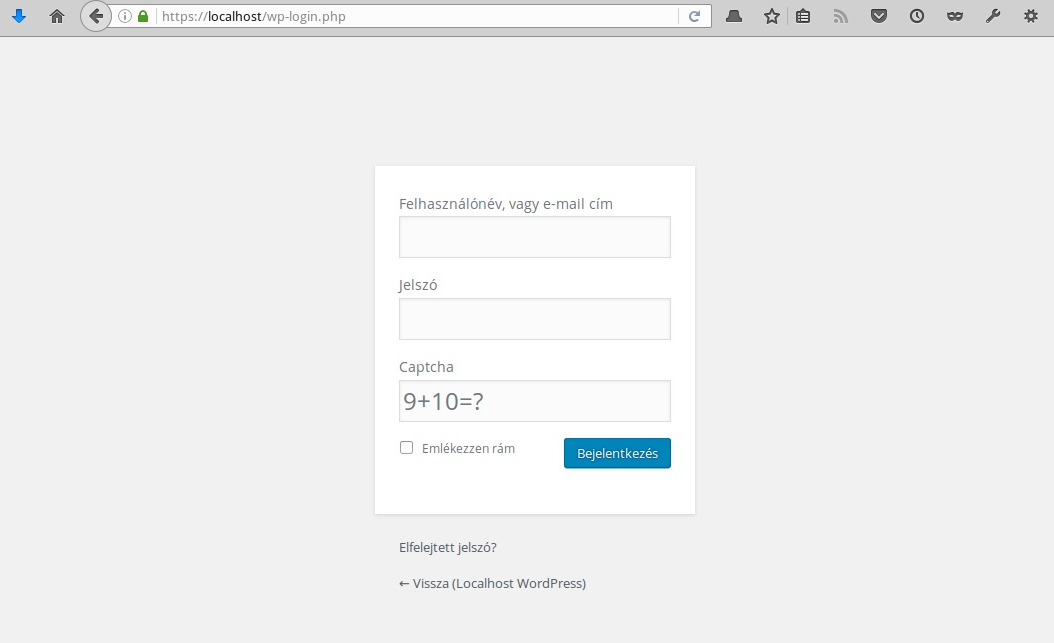
\includegraphics[width=1\textwidth]{wp-login-url.jpg}
	\caption{A bejelentkezési felület}
\end{figure}

A WordPress az adminisztrációs felületen feltöltött fájlokat alapértelmezetten a \texttt{/wp-content/uploads} mappába helyezi el, s bár alapvetően a Médiatárban feltölthető fájlok típusa korlátozva van, ettől még célszerű védekezni más típusú fájlok futtathatósága ellen. Ezért a jelölt mappában egy \texttt{.htaccess} fájlban az alábbi kódot helyeztem el, mely kizárólag a felsorolt kiterjesztésű fájlokat engedi olvasni:

\begin{lstlisting}
order deny,allow
deny from all
<files ~ ".(xml|css|jpe?g|png|gif|js)$">
	allow from all
</files>
\end{lstlisting}

A WordPress egy újabb kritikus pontja a felhasználónevek könnyű kinyerése, ugyanis az alap URL-hez társított \texttt{?author=[userID]} (itt a userID egy egész szám egytől kezdve, a meglévő felhasználók számáig bezárólag, lényegében a felhasználó adatbázis azonosítója) átirányít a felhasználó bejelentkezési nevéből (úgynevezett nickname) képzett URL-re (\texttt{/author/[username]}). Mivel a rendszer nyílt forráskódú, így a bejelentkezési felület elérhetősége mindenki (köztük hackerek) számára ismert, a felhasználónevek pedig így kinyerhetőek, ezért célszerű a WordPress ezen átirányítási funkcióját tiltani. Az erre szolgáló, bővítményben elhelyezett kód a következő, mely a \verb|?author=| kéréseket átirányítja a főoldalra:

\begin{lstlisting}
// redirects ?author= URLs to homepage to avoid getting author names
add_action('template_redirect', 'HideAuthorURL');
function HideAuthorURL()
{
	if (is_author())
	{
		wp_redirect(home_url());
		exit;
	}
}
\end{lstlisting}

A WordPress alapértelmezetten tartalmaz egy adminisztrációs felületről elérhető szerkesztőfelületet a bővítmények és sablonok fájljainak módosítására, azonban ez szintúgy biztonsági kockázatot jelent, ezért ezt letiltottam a \texttt{wp-config.php} fájlban elhelyezett alábbi kód segítségével:

\begin{lstlisting}
define('DISALLOW_FILE_EDIT', true);
\end{lstlisting}

A szintúgy ezen konfigurációs fájlban található \texttt{\$table\_prefix} változó értékét az eredeti \texttt{wp\_}-ról szintúgy megváltoztattam \texttt{ccrmswp\_}-re, hiszen a rendszer nyílt forráskódú mivolta miatt ez egy újabb biztonsági rés. Természetesen célszerű ennél bonyolultabb, randomgenerált prefixet használni.

A WordPress egy ingyenes, nemzetközi közösség által készített és folyamatosan továbbfejlesztett tartalomkezelő, ám az újítások nem kerülnek be automatikusan a rendszerbe, hanem SVN szerverekről tölthetőek le, akár csomagolt formátumban is. Ez egyik oldalról jó, hisz egy-egy bevezetett újítás vagy módosítás gondot okozhat egy korábban elkészített oldalnál, másrészt hátrány, hiszen így a szükséges (biztonsági) javítások sem települnek.

Ezért az alábbi kódokat a \texttt{wp-config.php} fájlban szintúgy célszerű elhelyezni, mely biztosítja az alaprendszer automatikus frissítését.

\begin{lstlisting}
// enable automatic update
define('WP_AUTO_UPDATE_CORE', true);
\end{lstlisting}

Emellett a harmadik fél által fejlesztett sablonok és bővítmények szintúgy SVN-ről tölthetőek le, melyek automatikus frissítése természetesen ugyanúgy ajánlott, melyet a pluginban elhelyezett alábbi kóddal biztosítok:

\begin{lstlisting}
// enable automatic updates for plugins
add_filter('auto_update_plugin', '__return_true');

// enable automatic updates for themes
add_filter('auto_update_theme', '__return_true');
\end{lstlisting}

A WordPress tartalomkezelővel készült honlapokat rengeteg támadás éri, hiszen lényegében rengeteg módszerrel leellenőrizhető automatikusan, hogy az adott weboldal motorja ismert CMS-e, ha igen, pontosan melyik az. Így például a \verb|wp-admin|, \verb|wp-login.php| fájlok megléte (200-as válaszüzenet a szervertől ezek lekérésekor), valamint a WP a website \texttt{<head>} részébe is elhelyez egy \texttt{<meta name="generator" content="WordPress" />} tagot. Ezt célszerű is eltávolítani, erre a WordPress szintúgy biztosít lehetőséget:

\begin{lstlisting}
// hide generator from header
remove_action('wp_head', 'wp_generator');
\end{lstlisting}

\Section{Többnyelvűsítés - iln18}

Az \texttt{iln18} egy nemzetközi jelzése a többnyelvűsítésnek, mely arra utal, hogy az \texttt{l} és \texttt{n} karakterek között nemzetközi viszonylatban összesen 18 másik karakter létezik. Bár a magyar nyelvben csak az \verb|ly| és \verb|m| foglal helyet, de nem feledkezhetünk meg más országok, népek nyelvéről sem.

A rendszer többnyelvűsítésére a WordPress-nél megismert PO/MO megoldást választottam, ahol a \texttt{.po} fájl a Portable Object, a \texttt{.mo} a Machine Object, azaz az elsőbe a fordítandó és a fordított szöveg kerül, míg a másodikba már gépi kódra fordított változat. Az fordítandó szövegek kiindulási állapotát egy \texttt{.pot} fájlba szokás összefoglalni. A PHP nyelvben ezen megoldás kezelésére a \texttt{gettext} függvénykönyvtár szolgál.

A \texttt{.po} tartalma kötelezően (természetesen az egyes megnevezések átírandóak):

\begin{lstlisting}
msgid ""
msgstr ""
"Project-Id-Version: CCRMS\n"
"Report-Msgid-Bugs-To: http://users.iit.uni-miskolc.hu/~harkaly/\n"
"POT-Creation-Date: 2016-01-30 01:00+0100\n"
"PO-Revision-Date: 2016-01-30 01:00+0100\n"
"Last-Translator: Harkály Gergő <harkaly@iit.uni-miskolc.hu>\n"
"Language-Team: Harkály Gergő <harkaly@iit.uni-miskolc.hu>\n"
"Language: hu\n"
"MIME-Version: 1.0\n"
"Content-Type: text/plain; charset=UTF-8\n"
"Content-Transfer-Encoding: 8bit\n"
\end{lstlisting}

Megjegyzéseket a \texttt{\#} jellel lehet elhelyezni, például a shell fordítási parancsot segítségképpen: \texttt{\#msgfmt textdomain-hu\_HU.po -o textdomain-hu\_HU.mo}

A fordítandó szövegeket a \texttt{msgid}, az adott nyelv megfelelőjét pedig a \texttt{msgstr} kulcsszavakkal kell meghatározni az alábbiakhoz hasonló formában:

\begin{lstlisting}
msgid "username"
msgstr "felhasználónév"

msgid "password"
msgstr "jelszó"
\end{lstlisting}

A két fájltípust egy \texttt{lang} (vagy languages) mappában célszerű elhelyezni, majd ezekre a fájlokra mind a sablonban (functions.php fájl), mind a bővítményben hivatkozni kell, melyre szintúgy van WordPress funkció:

\begin{lstlisting}
// load translated text for plugin
load_plugin_textdomain('ccrmsplugin', false, dirname(plugin_basename(__FILE__)).'/lang/');
// load translated text for theme
load_theme_textdomain('ccrmstheme', get_template_directory() . '/lang');
\end{lstlisting}

Fentebb látható is, hogy megjelent a korábban már említett \verb|textdomain|, melyet a fordítandó szövegek használatakor kell alkalmazni. A fordítási egységek megadásakor az első paraméter mindig a sablon vagy bővítmény \verb|textdomain| értéke, második pedig a fordítási fájlokat (.po, .mo) tartalmazó mappa elérési útvonala.

\Section{Saját fejlesztésű funkciók}

Bár a WordPress számos funkciót biztosít, melyekkel egy összetettebb honlapot is létre lehet hozni, mégis úgy gondoltam, a kódújrafelhasználás miatt célszerű néhány saját függvényt is definiálni.

Szerettem volna felkészülni a többnyelvűsítésre is, melyben a feltételezés az, hogy az egyes nyelvekhez tartozó oldalak URL-jében a fődomain mögött az adott nyelv két karakterből álló rövidített verziója fog majd szerepelni, például \texttt{domain.hu/en/}, \texttt{domain.hu/de/}. A megalkotott függvény segítségével először a link végének levágásával meghatározom az adott nyelvet, majd arra alapozva további konstans értékeket, hiszen a HTML tagok valamint különböző API-k \verb|lang| paramétere eltérhet (például hu-HU vagy hu\_HU). Nehezítette a dolgot, hogy az angol nyelv kétbetűs kódja egyértelműen az \texttt{en}, azonban például a \texttt{hu\_HU} és \texttt{de\_DE} meghatározáshoz hasonlóan nincs \texttt{en\_EN}, de van \texttt{GB} vagy \texttt{US}. Egyelőre a \texttt{GB} verzió mellett döntöttem.

\newpage

\begin{lstlisting}
// set locale variable based on URL substring
function SetLocaleByURL()
{
	$URLlang = substr(\$_SERVER['REQUEST_URI'], 1, 2);
	if($URLlang==='en')
	{
		$URLLANG = 'GB';
	}
	else
	{
		$URLLANG = strtoupper($URLlang);
	}
	define('locale', $URLlang);
	define('locale-LOCALE', $URLlang.'-'.$URLLANG);
	define('locale_LOCALE', $URLlang.'_'.$URLLANG);
	return;
}
\end{lstlisting}

Egy-egy oldal teljes URL-jének lekérése:

\begin{lstlisting}
// get current page full URL
function getFullURL()
{
	return 'http'.(isset($_SERVER['HTTPS']) ? 's' : '').'://'.$_SERVER['HTTP_HOST'].$_SERVER['REQUEST_URI'];
}
\end{lstlisting}

\Section{Sablon létrehozása}

A WordPress sablon számos fájlból épül fel a következők szerint:

\begin{itemize}
	\item 404.php - 404 hiba oldal sablonja
	\item archive.php - több speciális kategória sablonja, például a dátum szerinti rendezés esetében
	\item author.php - adott bejegyzést író adatlapjának sablonja
	\item category.php - kategóriák sablonja
	\item comments.php - hozzászólást biztosító űrlap és meglévő hozzászólások megjelenítésére szolgál, elhagyható
	\item footer.php - lábléc sablonja
	\item functions.php - mind a külső, mind a belső (admin panel) funkciók megadására szolgál, elhagyható
	\item header.php - a sablon fejlecének kódjait tartalmazza
	\item index.php - kezdőoldal beállítása
	\item page.php - Oldal sablonminta
	\item page\_egyedi.php - egyedi Oldal sablonminta is alkotható
	\item screenshot.png - admin panelben a választható sablonoknál megjelenő kép
	\item search.php - keresési eredmények megjelenítésére szolgál, elhagyható
	\item sidebar.php - oldalsáv sablonminta
	\item single.php - Bejegyzés sablonminta
	\item style.css - legfőképpen a sablon adatait tartalmazza
	\item tag.php - címke sablonminta
\end{itemize}

A sablon optimális működéséhez számos funkciót kell deklarálni annak mappájában (\texttt{/wp-content/themes/CCRMS-theme}) található \texttt{functions.php} fájlban.

Ahhoz, hogy a bejegyzésnél legyen lehetőség kapcsolódó, kiemelt kép feltöltésére, illetve annak a weboldalon történő megjelenítésére, az alábbi kódot kell elhelyezni a fent jelölt funkciókat tartalmazó fájlban:

\begin{lstlisting}
// add theme post thumbnail support
add_theme_support('post-thumbnails');
\end{lstlisting}

2016-ban értelmetlennek tűnik olyan honlapot készíteni, amely nincs felkészítve a közösségi oldalakra, így az ehhez szükséges metaadatokat is beépítettem a sablonba. A \href{https://developers.facebook.com/docs/sharing/webmasters}{Facebook Open Graph}-ra alapozva, a WordPress függvényeit kihasználva helyeztem el a sablon \texttt{header.php} fájljában azt a kódot, mely a mellékletben megtalálható. \ref{Chap:melleklet}

A \href{https://dev.twitter.com/cards/overview}{Twitter Cards} hasonló elven működik, a kapcsolódó meta tagokat szintúgy a \texttt{header.php}-ban kell elhelyezni:

\begin{lstlisting}
	<!-- Twitter Cards | https://dev.twitter.com/cards/overview -->
	<meta name="twitter:card" content="summary" />
	<meta name="twitter:site" content="@" />
	<meta name="twitter:title" content="<?php wp_title(''); ?>" />
	<meta name="twitter:description" content="<?php if(is_home()) { bloginfo('description'); } else { getPostExcerptOutsideLoop($post->ID, 160, FALSE); } ?>" />
	<meta name="twitter:image" content="<?php if(has_post_thumbnail($post->ID)) echo wp_get_attachment_image_src(get_post_thumbnail_id($post->ID), 'medium')['0']; ?>" />
\end{lstlisting}

A Pinterestnél csupán egyetlen sor szükséges a weboldal igazolásához:

\begin{lstlisting}
	<!-- Pinterest domain verify -->
	<meta name="p:domain_verify" content="<?=get_theme_mod('pinterestDomainVerifyID');?>">
\end{lstlisting}

A Google keresőoptimalizálást segítő egyik eszköze a \href{https://www.google.com/webmasters/tools/home?hl=HU}{Search Console}, a hozzá tartozó információk meta tagja:

\begin{lstlisting}
	<!-- Google Search Console -->
	<meta name="google-site-verification" content="">
\end{lstlisting}

\Section{A Bootstrap bemutatása}

Manapság elengedhetetlen a reszponzív megjelenés, azaz ahogy azt mondani szokták: kijelzőfüggetlen megjelenés, bár én pont hogy kijelzőfüggőnek nevezném. Mitöbb, a \href{https://webmasters.googleblog.com/2015/02/finding-more-mobile-friendly-search.html}{Google rangsorolási algoritmusának része lett 2015. április 21-től}, így a mobilos keresések során azok a weboldalak, melyek nincsenek felkészítve a kisebb kijelzőméretekre, hátrányos megkülönböztetésben részesülnek. (Itt megjegyezném, hogy 2016-ra még ennél is komolyabb változásokat helyeztek kilátásba a legnagyobb technológia cégek az \href{https://www.ampproject.org/}{Accelerated Mobile Pages Project} keretében, hogy még jobban növelni tudják a mobilos felhasználói élményt.)

A kijelzőfüggetlen megjelenés kialakításához a \href{http://getbootstrap.com/}{Boostrap}et választottam. A Bootstrap a legnépszerűbb HTML, CSS és JS keretrendszer reszponzív, úgynevezett ``mobile first'' projektek megalkotásához. A mobile first kifejezés egy szemléletmód, mely arra utal, hogy a projekt megvalósítása során a mobilos megjelenés kerül előtérbe, s nem a teljes képernyőre helyeződik a fókusz, ezért igyekszik minimalizálni a szükséges kódokat, hiszen egy mobiltelefon nyilván kisebb memória és processzor kapacitással rendelkezik, nem beszélve a mobilnet sebességéről.

A Bootstrap egy sort 12 oszlopra oszt fel (col-*-*), s ezeket a részeket tehetjük egymás mellé, alá. Emellett négy méretben gondolkodik, melyeket az \verb|xs, sm, md, lg| kulcsszavak jelölnek, tehát egy egység oszlopainak száma akár a mobil, tablet, PC függvényében deklarálhatóak, például: \texttt{col-sm-12}, \texttt{col-md-8}, \texttt{col-lg-4}.

Mivel a WordPress alapvetően nem Bootstrapre építkezik a sablonok esetében, így szükség volt a menüsáv kialakításánál egy már kész komponens használatára: \url{https://github.com/twittem/wp-bootstrap-navwalker}

\newpage

\Section{Felhasználói elégedettség növelése}

\SubSection{Keresőmező}

A WordPress-nek van beépített funkciója a Bejegyzésekhez/Oldalakhoz való hozzászólásra, ám a kéretlen kommentek (spam) elkerülése végett célszerű ezt regisztrációhoz kötni. Tekintettel arra, hogy a Facebook jelentősen az emberek életévé vált, ezért integráltam a \href{https://developers.facebook.com/docs/plugins/comments/}{Facebook Comments Plugin}t. Emellett egy másik szolgáltatás is egyre nagyobb teret nyer az online világban a hozzászólások esetében, mégpedig a \href{https://disqus.com/}{Disqus}. A bejegyzések alatt megjelenő hozzászólási lehetőségnél tehát három opció megjelenik a következő sorrendben: Disqus, Facebook, (WordPress) fiókkal rendelkezőknek.

\begin{figure}
	
\includegraphics[width=1\textwidth]{comment-block.jpg}
	\caption{Hozzászólási lehetőség a bejegyzések alatt}
\end{figure}

\SubSection{Marketing}

\tab\textbf{CTO gomb}

CTO, azaz call-to-action gomb, mely azonnali cselekvésre ösztönöz, ennek cél linkje, valamint a felirata tetszőlegesen módosítható (például Hívjon most!, Kérjen útirányt a bolthoz!, Vásároljon most!).

\newpage

\textbf{Megosztógombok}

Napjainkban az online marketing elkerülhetetlen eleme a közösségi oldalak kihasználása, lényegében a weboldal felhasználóinak segítségével költségmentesen juthat el új személyekhez egy-egy tartalom, legyen az blogbejegyzés, vagy egy webshop terméke. Ezért automatikusan megjelentetek négy gombot a bejegyzések végén népszerűségi sorrendben: Facebook, Twitter, Google Plus és Nyomtatás. A Facebooknál a Facebook API segítségével azt is lekérdezem, hogy az adott bejegyzést hányszor osztották meg összesen.

\begin{lstlisting}
// display share buttons after posts
function ShareButtons()
{
	// Facebook stat number
	$FacebookJSON = json_decode( file_get_contents( 'https://api.facebook.com/method/links.getStats?urls=' . getFullURL().'&format=json' ), true);
	?>
	<div class="row text-center">
		<p style="text-align:center;"><i>Ha szerinted másokat is érdekelhet ez a cikk, akkor oszd meg velük!</i></p>
		<a target="_blank" rel="nofollow" href="https://www.facebook.com/sharer/sharer.php?u=<?php the_permalink() ?>" class="btn btn-primary btn-xs"><span class="glyphicon glyphicon-share-alt"></span> <span class="hidden-xs">Megosztás Facebookon (<?=$FacebookJSON['0']['total_count'];?>)</span></a>
		<a target="_blank" rel="nofollow" href="https://twitter.com/home?status=<?php the_permalink() ?>" class="btn btn-info btn-xs"><span class="glyphicon glyphicon-share-alt"></span> <span class="hidden-xs">Megosztás Twitteren</span></a>
		<a target="_blank" rel="nofollow" href="https://plus.google.com/share?url=<?php the_permalink() ?>" class="btn btn-danger btn-xs"><span class="glyphicon glyphicon-share-alt"></span> <span class="hidden-xs">Megosztás Google Plus-on</span></a>
		<a onclick="window.print();" class="btn btn-default btn-xs"><span class="glyphicon glyphicon-print"></span> <span class="hidden-xs">Nyomtatás</span></a>
	</div>
<?php }

\end{lstlisting}

\begin{figure}
	
\includegraphics[width=1\textwidth]{share-buttons.png}
	\caption{Megosztogombok a bejegyzések végén}
\end{figure}
%\include{sajat}
\Chapter{Összefoglalás}
\label{Chap:osszefoglalas}

\Section{Magyar}

A létrejött webalkalmazás összességében megfelel a mai kor igényeinek, hiszen a sokoldalú adminisztrációs felület, a reszponzív megjelenés, valamint a közösségi oldalak integrációja mind-mind hozzájárul egy vállalkozás sikeres online jelenlétéhez.

A feladat kivitelezése során sikerült mélyebben elsajátítani a WordPress rendszer használatát, megismerni a hozzá kapcsolódó WooCommerce bővítményt, valamint a Twitter által fejlesztett Bootstrap keretrendszert is. Mindez a tudás jelenleg rendkívül hasznos, hisz az informatikai piacon ezek a technológiák vezető szerepet töltenek be a saját területükön.

A rendszer azonban még korántsem tökéletes, számos ponton lehetne még javítani. Ezek közül a legfontosabbak:

\begin{itemize}
	\item \textbf{breadcrumbs}: a kifejezésnek magyar egységesített megfelelője még nincs, talán a webmorzsa szó a legtalálóbb. A breadcrumbs egy navigációs eszköz, mely a weboldal kiindulópontjától (például domain.hu/) a felhasználó aktuális tartózkodási helyéig (például domain.hu/termekek/ferfi-ruha/nadrag/kek-feher-csikos-farmer) vezető utat mutatja (például Főoldal > Termékek > Férfi ruha > Nadrág > Kék-fehér csíkos farmer)
	\item \textbf{microformats}: a mikroformátum olyan adatforma, melyeket különböző adattípusok egységesítésére használnak. A mikroformátum a keresőrobotok, azaz az úgynevezett "bot"-ok és az emberek számára is értelmezhető és olvasható adat. Funkciója, hogy az egységes forma révén az adatok kereshetővé, valamint más alkalmazásokba is egyszerűen beilleszthetőekké válnak.  További részletek angol nyelven a \url{http://microformats.org/} oldalon érhetőek el.
	\item \textbf{schema tag}: a schema jelölések használata webáruházaknál, de bármilyen weboldalnál szinte már kötelező, hiszen ezzel is nagyobb forgalom generálható a keresők találati listáján, illetve annak különböző kiegészítéseinél. A felhasználók számára így hasznosabbá, érthetőbbé válik a kínált tartalom, javul a felhasználó élmény, amit a Google is értékel. További részletek angol nyelven a \url{https://schema.org/} oldalon érhető el.
\end{itemize}

A \href{https://developers.google.com/structured-data/testing-tool/}{Google fejlesztői felületén} lehetőség van tesztelni is ezeket az adatokat.

\Section{English}

The created webb application meets the nees of today, as the versatile administrative interface (dashboard), responsive appearance (layout) and social networking integration all contribute to a successful online business presence.

While I've been performing tasks I could learn to use WordPress system, know the associated plugin named WooCommerce and the Bootstrap framework developed by Twitter. This knowledge is currently very useful, because in the IT market these technologies are leaders in their respective territories.

The system is far from perfect, however, a number of points could be improved. The most important are:

\begin{itemize}
	\item \textbf{breadcrumbs}: there isn't a perfect Hungarian translate for it, maybe it could be named "webmorzsa". The breadcrumbs is a navigation tool which shows the way on the webpage from the website's root (for example domain.hu/) to the current position (for example domain/hu/shop/product/men/jeans/blue-white-stripped-jeans) in this format: Homepage > Shop > Producst > Men > Jeans > Blue-white stripped jeans.
	\item \textbf{microformats}: Microformats are data formats which used for unifies different data types. The microformats are interpretable and readable for search bots and people too. It's function is to unified data type could be searchable and pastable into apps. More information in English on the \url{http://microformats.org/} site.
	\item \textbf{schema tag}: usage of schema on webshops or any other type of webpage is a must nowadays, because higher traffic can be generated on search results' page and on that's other plugins. In this way the content is more useful and understandable for users, user experience improves, what Google appreciates too. More information on the \url{https://schema.org/} site.
\end{itemize}

On the \href{https://developers.google.com/structured-data/testing-tool/}{Google' developers site} this tools can be tested.

\newpage

\Chapter{Mellékletek}
\label{Chap:melleklet}

\Section{Forráskódok}

\newpage

\SubSection{Facebook Open Graph kódja a sablon header.php-ban}

\begin{lstlisting}
	<!-- Facebook OpenGraph | https://developers.facebook.com/docs/sharing/best-practices -->
	<meta property="fb:app_id" content="837847339665576">
	<meta property="og:url" content="<?=getFullURL();?>">
	<meta property="og:title" content="<?php wp_title(''); echo ' - '; bloginfo('name'); ?>">
	<meta property="og:site_name" content="<?php bloginfo('name'); ?>">
	<meta property="og:description" content="<?lphp if(is_home()) { bloginfo('description'); } else { echo getPostExcerptOutsideLoop($post->ID, 160, FALSE); } ?>">
	<meta property="og:locale" content="<?=$locale.locale_LOCALE;?>">
	<?php global $pagenow; if(is_single()) { ?>
		<meta property="og:type" content="article">
		<meta property="og:image" content="<?php if(has_post_thumbnail($post->ID)) echo wp_get_attachment_image_src( get_post_thumbnail_id($post->ID ), 'medium')['0']; ?>">
		<meta property="article:author" content="<?=get_theme_mod('facebookpageURL');?>">
		<meta property="article:publisher" content="<?=get_theme_mod('facebookpageURL');?>">
		<meta property="article:published_time" content="<?=get_the_date('Y-m-d H:i:s'); the_date('Y-m-d H:i:s'); ?>">
		<meta property="article:modified_time" content="<?php the_modified_date('Y-m-d H:i:s'); ?>">
		<!--<meta property="article:expiration_time" content="">-->
		<meta property="article:section" content="">
		<meta property="article:tag" content="<?php $posttags=get_the_tags(); if($posttags) { foreach($posttags as $tag) { echo $tag->name.', '; } } ?>">
	<?php
	} elseif ($pagenow == 'product.php') {
	?>
		<meta property="product:plural_title" content="-">
		<meta property="product:price:amount" content="100">
		<meta property="product:price:currency" content="HUF">
	<?php
	} elseif ($pagenow == 'profile.php') {
		?>
		<meta property="og:type" content="profile">
		<meta property="profile:first_name" content="">
		<meta property="profile:last_name" content="">
		<meta property="profile:username" content="">
		<meta property="profile:gender" content="">
	<?php
	} else {
		?>
		<meta property="og:type" content="website">
	<?php } ?>
\end{lstlisting}

\newpage

\SubSection{A captcha kódja}

\begin{lstlisting}
// captcha on login form
class LoginFormCaptcha
{
	private $key1, $key2;
	public function __construct()
	{
		add_action('login_form', array($this, 'captcha_display'));
		add_action('wp_authenticate_user', array($this, 'validate_captcha'), 10, 2);
	}
	public function captcha_display()
	{
		$key1 = rand(1,10);
		$key2 = rand(1,10);
		?>
			<p>
				<label for="user_captcha">Captcha</label>
				<input type="text" name="user_captcha" class="input" placeholder="<?=$key1.'+'.$key2.'=?';?>" required>
				<input type="hidden" name="captcharesult" value="<?=$key1+$key2;?>" required>
			</p>
	<?php }
	public function validate_captcha($user, $password)
	{
		if(!isset($_POST['user_captcha']) || empty($_POST['user_captcha']) || !isset($_POST['captcharesult']) || empty($_POST['captcharesult']))
		{
			return new WP_Error('empty_captcha', __('CAPTCHA should not be empty', 'ccrmsplugin'));
		}
		if(isset($_POST['user_captcha']) && isset($_POST['captcharesult']) && $_POST['user_captcha'] != $_POST['captcharesult'])
		{
			return new WP_Error('invalid_captcha', __('CAPTCHA response was incorrect', 'ccrmsplugin'));
		}
		return $user;
	}
}
new LoginFormCaptcha();
\end{lstlisting}

\newpage

\Section{Képek}

\begin{figure}[H]
	\centering
		
\includegraphics[height=8.5in]{katt-sport-hu-teljes-fooldal.jpg}
		\caption{A katt.sport.hu főoldala}
\end{figure}

\begin{figure}[H]
	\centering
		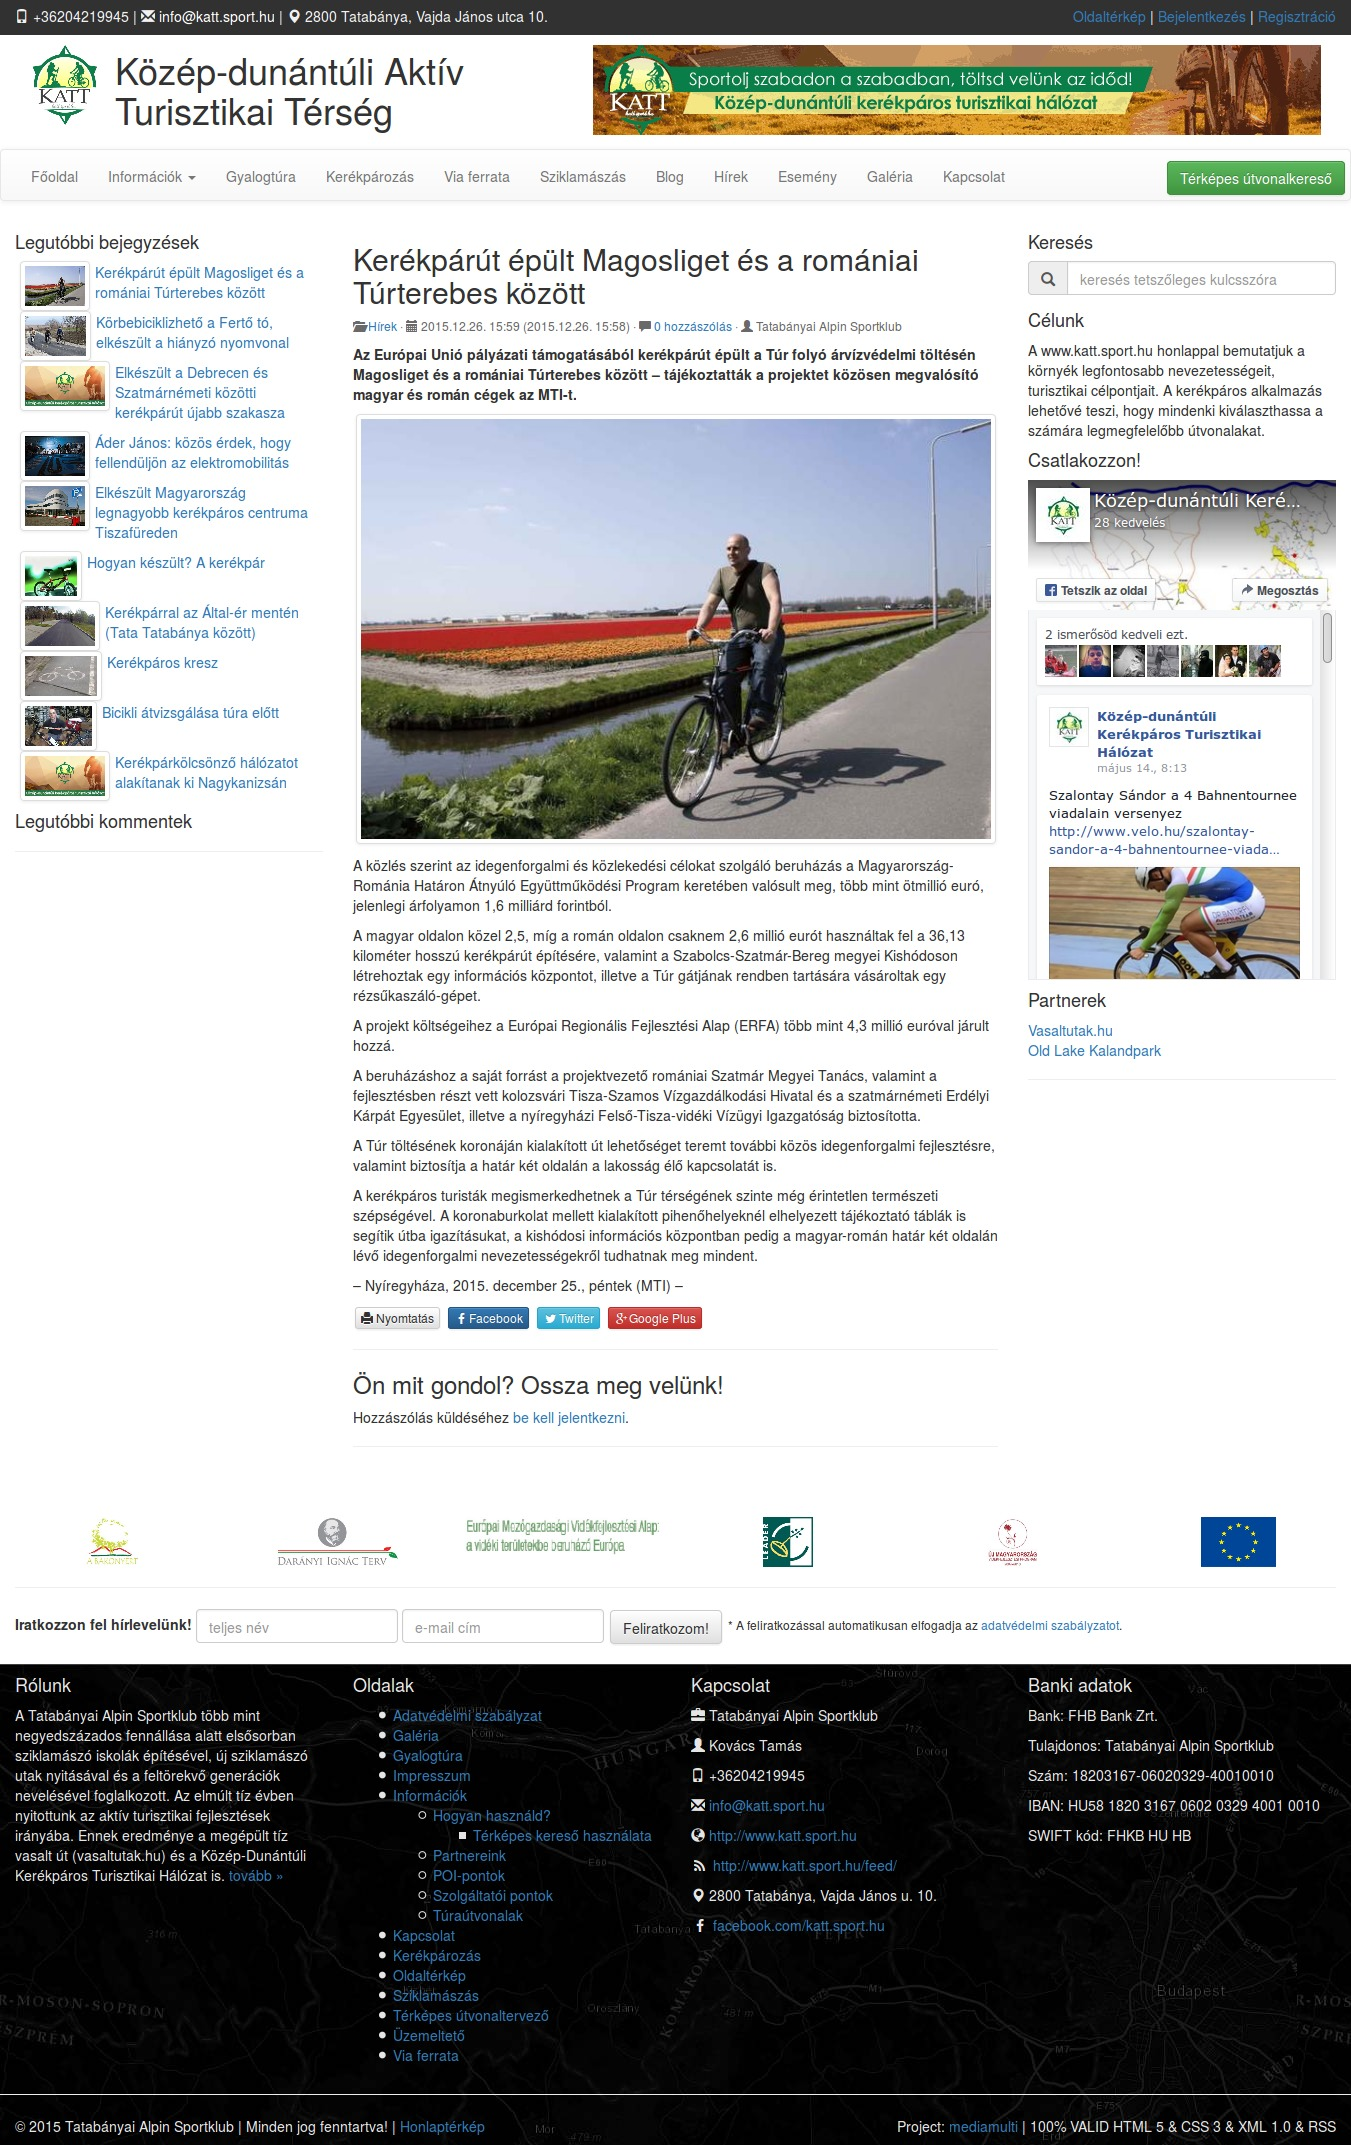
\includegraphics[height=8.5in]{katt-sport-hu-bejegyzes.jpg}
		\caption{Példa a katt.sport.hu bejegyzésének megjelenítésére}
\end{figure}

\newpage
\begin{thebibliography}{x}
	\addcontentsline{toc}{chapter}{\bibname}
	\bibitem{Drupal} Drupal: \url{https://www.drupal.org/}
	\bibitem{Joomla} Joomla: \url{https://www.joomla.org/}
	\bibitem{Magento} Magento: \url{http://magento.com/}
	\bibitem{OpenCart} OpenCart: \url{http://www.opencart.com/}
	\bibitem{PrestaShop} PrestaShop: \url{https://www.prestashop.com/}
	\bibitem{MiniCRM} MiniCRM: \url{http://www.minicrm.hu/}
	\bibitem{TrilobitaSiebel} Oracle Siebel Crm | Trilobita Informatics Excl. Co.: \url{http://www.trilobita.hu/termekek/viszonteladott-termekek/oracle-alkalmazasok/oracle-siebel-crm}
	\bibitem{WordPress} WordPress: \url{http://wordpress.org/}, \url{http://wordpress.com/}
	\bibitem{MiniCRM} MiniCRM: \url{http://www.minicrm.hu/tour/crm/}
	\bibitem{Automattic} Automattic: \url{https://automattic.com/}
	\bibitem{FacebookOpenGraph} Facebook Open Graph: \url{https://developers.facebook.com/docs/sharing/webmasters}, \url{http://ogp.me/}
	\bibitem{TwitterCards} Twitter Cards: \url{https://dev.twitter.com/cards/overview}
	\bibitem{Bootstrap} Bootstrap: \url{http://getbootstrap.com/}
	\bibitem{Schema} Schema.org: \url{https://schema.org/}
	\bibitem{Microformats} Microformats: \url{http://microformats.org/}
	\bibitem{FpsMicroformats} Mikroformátumok és SEO | FPS blog: \url{http://blog.fps.hu/post/36584399122/mikroformatumok-seo}
	\bibitem{GoogleSearchConsole} Google Search Console: \url{https://www.google.com/webmasters/tools/home?hl=HU}
	\bibitem{ShopRenter} ShopRenter.hu \url{https://www.shoprenter.hu/}
	\bibitem{WikipediaPrestaShop} PrestaShop | Wikipédia: \url{https://hu.wikipedia.org/wiki/PrestaShop}
	\bibitem{Google20150421} Google Webmaster Central Blog: \url{https://webmasters.googleblog.com/2015/02/finding-more-mobile-friendly-search.html}
	\bibitem{AMP} Accelerated Mobile Pages Project: \url{https://www.ampproject.org/}
	\bibitem{WPBSNAV} wp-bootstrap-navwalker: \url{https://github.com/twittem/wp-bootstrap-navwalker}
	\bibitem{FBcomments} Facebook Comments Plugin: \url{https://developers.facebook.com/docs/plugins/comments/}
	\bibitem{Disqus} Disqus: \url{https://disqus.com/}
	\bibitem{GoogleStrucuredData} Google Struktúrált adatok teszteszköze: \url{https://developers.google.com/structured-data/testing-tool/}
	\bibitem{phparray} PHP tömbkezelés: \url{http://php.net/manual/en/language.types.array.php}
\end{thebibliography}
%Az összefoglaló fejezet
\chapter*{Adathordozó használati útmutató}
\addcontentsline{toc}{chapter}{Adathordozó használati útmutató}

A mellékelt adathordozón a \texttt{SERVER} mappában található fájlokat szükséges felmásolni a kívánt webszerverre, de természetesen localhostra is telepíthető a csomag. A \texttt{public\_html} mappában lesznek azok a fájlok, melyek a domain név gyökérkönyvtárába kerülnek, a mellette található \texttt{.htpasswd} fájl pedig biztonsági okokból egy szinttel feljebb helyezendő el. A csomag tartalmazza a WordPress 2016. május 12-én aktuális, 4.5.2-es, valamint a WooCoomerce 2.5.5-ös változatát, emellett az általam készített sablon és plugin fájljait is, valamint egyéb kiegészítőket.

 A \texttt{public\_html/wp-admin/.htaccess} fájlban a \texttt{.htpasswd} abszolút elérési útvonalát szükséges megadni a \texttt{AuthUserFile /path/to/.htpasswd} helyen.

A telepítéshez első körben létre kell hozni egy MySQL adatbázist a szerveren, melyre a phpMyAdmin segítségével grafikus felületen is lehetőség van, amennyiben az jelen van az adott tárhelyen. Ezt követően a telepítés már egyszerű, hiszen csak meg kell hívni böngészőben az URL-t, mely alá be lettek másolva a fájlok (például http://localhost vagy http://www.domain.hu), s azonnal megjelenik egy telepítési útmutató, melyet értelemszerűen kell kitölteni, például a létrehozott adatbázis információival.

Sikeres telepítést követően megjelenik az adminisztrációs felület. A bal oldalsávban találhatóak a menüpontok, a \verb|Megjelenés  > Sablonok|  almenü alatt az egyes sablonok, a \verb|Bővítmények > Telepített bővítmények| almenü alatt az egyes pluginok kapcsolhatóak be, vagy a későbbiekben ki. Ezután a \texttt{Beállítások}, valamint a \texttt{WooCommerce} menüpontokon belül számos lehetőség van módosítani a rendszert.

Új szöveges tartalmakat a \texttt{Bejegyzések}, valamint az \texttt{Oldal}, termékeket a \texttt{Termékek} menüpontokon belül lehet felvinni, illetve a későbbiekben a meglévőeket módosítani.

A \verb|public_html| mappa mellett elhelyeztem egy \verb|demo.sql| fájlt is, melyet a MySQL-be importálva (például phpMyAdminon keresztül) egy tesztadatokkal feltöltött környezett kapunk.
\end{document}